%% pc-lewis-molecules — schémas de Lewis de quatre molécules.
%% Les doublets (liants et non liants) sont tous représentés par des TIRETS.
%% Un doublet non liant est posé par \dnl{<atome>}{<angle>}{<distance>} : le tiret
%% est tracé perpendiculairement à la direction donnée, comme dans le manuel.
\documentclass[tikz,border=4pt]{standalone}
\usepackage{liaisons}
\usetikzlibrary{shapes.geometric, positioning}
\begin{document}
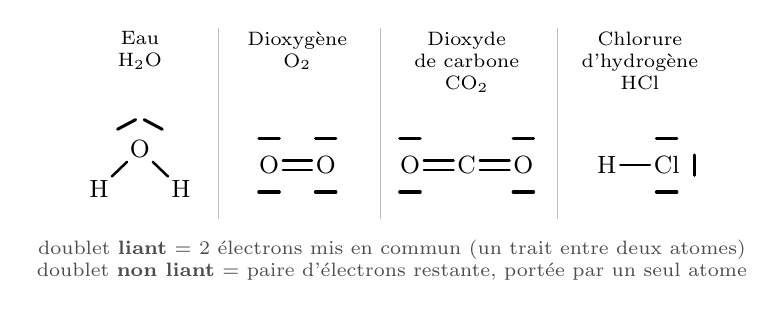
\begin{tikzpicture}[x=1cm,y=1cm,
  atome/.style={inner sep=1.2pt, font=\small},
  lien/.style={line width=0.9pt, line cap=round},
  entete/.style={font=\scriptsize, align=center, anchor=north, text width=1.8cm, inner sep=1pt},
  filet/.style={line width=0.4pt, draw=black!25}]

%% doublet non liant : \dnl{(x,y) de l'atome}{angle}{distance}
\newcommand\dnl[3]{\begin{scope}[shift={#1}, rotate=#2]
  \draw[line width=1.1pt, line cap=round] (#3,-0.13) -- (#3,0.13); \end{scope}}

%% ================= Eau : molécule coudée ==================================
\begin{scope}[shift={(0,0)}]
  \node[entete] at (0,1.12) {Eau\\$\mathrm{H_2O}$};
  \node[atome] (O)  at (0,-0.42)     {$\mathrm{O}$};
  \node[atome] (Ha) at (-0.52,-0.92) {$\mathrm{H}$};
  \node[atome] (Hb) at (0.52,-0.92)  {$\mathrm{H}$};
  \draw[lien] (O) -- (Ha);  \draw[lien] (O) -- (Hb);
  \dnl{(0,-0.42)}{62}{0.36}  \dnl{(0,-0.42)}{118}{0.36}
\end{scope}
\draw[filet] (1.00,1.12) -- (1.00,-1.30);

%% ================= Dioxygène : double liaison =============================
\begin{scope}[shift={(2.00,0)}]
  \node[entete] at (0,1.12) {Dioxygène\\$\mathrm{O_2}$};
  \node[atome] (O1) at (-0.36,-0.62) {$\mathrm{O}$};
  \node[atome] (O2) at (0.36,-0.62)  {$\mathrm{O}$};
  \draw[lien, transform canvas={yshift=1.7pt}]  (O1) -- (O2);
  \draw[lien, transform canvas={yshift=-1.7pt}] (O1) -- (O2);
  \dnl{(-0.36,-0.62)}{90}{0.34}  \dnl{(-0.36,-0.62)}{270}{0.34}
  \dnl{(0.36,-0.62)}{90}{0.34}   \dnl{(0.36,-0.62)}{270}{0.34}
\end{scope}
\draw[filet] (3.05,1.12) -- (3.05,-1.30);

%% ================= Dioxyde de carbone : molécule linéaire =================
\begin{scope}[shift={(4.15,0)}]
  \node[entete] at (0,1.12) {Dioxyde de carbone\\$\mathrm{CO_2}$};
  \node[atome] (Og) at (-0.72,-0.62) {$\mathrm{O}$};
  \node[atome] (C)  at (0,-0.62)     {$\mathrm{C}$};
  \node[atome] (Od) at (0.72,-0.62)  {$\mathrm{O}$};
  \foreach \d in {1.7,-1.7} {
    \draw[lien, transform canvas={yshift=\d pt}] (Og) -- (C);
    \draw[lien, transform canvas={yshift=\d pt}] (C) -- (Od);}
  \dnl{(-0.72,-0.62)}{90}{0.34}  \dnl{(-0.72,-0.62)}{270}{0.34}
  \dnl{(0.72,-0.62)}{90}{0.34}   \dnl{(0.72,-0.62)}{270}{0.34}
\end{scope}
\draw[filet] (5.30,1.12) -- (5.30,-1.30);

%% ================= Chlorure d'hydrogène : trois doublets sur Cl ===========
\begin{scope}[shift={(6.35,0)}]
  \node[entete] at (0,1.12) {Chlorure d'hydrogène\\$\mathrm{HCl}$};
  \node[atome] (H)  at (-0.42,-0.62) {$\mathrm{H}$};
  \node[atome] (Cl) at (0.34,-0.62)  {$\mathrm{Cl}$};
  \draw[lien] (H) -- (Cl);
  \dnl{(0.34,-0.62)}{90}{0.34}  \dnl{(0.34,-0.62)}{270}{0.34}
  \dnl{(0.34,-0.62)}{0}{0.35}
\end{scope}

%% ================= légende ================================================
\node[font=\scriptsize, text=black!70, align=center, anchor=north] at (3.2,-1.44)
  {doublet \textbf{liant} = 2 électrons mis en commun (un trait entre deux atomes)\\
   doublet \textbf{non liant} = paire d'électrons restante, portée par un seul atome};
\end{tikzpicture}
\end{document}
